\documentclass{article}[twocolumn]
\usepackage[pdftex]{graphicx}
\usepackage[utf8]{inputenc}
\usepackage[brazil]{babel}
\usepackage{subfigure}
\usepackage{mathtools}
\usepackage{amsmath}
\usepackage{amssymb}
\usepackage{float}
\usepackage{tikz}

\title{Lista 2}
\author{Kenji Yamane}

\begin{document}
	\maketitle
	\section{Quest\~ao 1}
	Calculando a jacobiana da EDO:
	\begin{equation}
		Df = \left[\begin{array}{cc}
			0 & 1\\
			1 - 2x + y & \mu + x
		\end{array}\right]
		\nonumber
	\end{equation}
	Aplicado em (0, 0):
	\begin{equation}
		Df(0, 0) = \left[\begin{array}{cc}
			0 & 1\\
			1 & \mu
		\end{array}\right]
		\nonumber
	\end{equation}
	Calculando os autovalores desta matriz:
	\begin{equation}
		\left|\begin{array}{cc}
			-\lambda & 1\\
			1 & \mu - \lambda
		\end{array}\right| = 0 \Rightarrow
		\nonumber
	\end{equation}
	\begin{equation}
		\Rightarrow \lambda^2 - \mu\lambda - 1 = 0 \Rightarrow
		\nonumber
	\end{equation}
	\begin{equation}
		\Rightarrow \lambda = \frac{\mu \pm \sqrt{\mu^2 + 4}}{2}
		\nonumber
	\end{equation}
	Calculando os autovetores:
	\begin{equation}
		\left[\begin{array}{cc}
			0 & 1\\
			1 & \mu
		\end{array}\right]
		\left[\begin{array}{c}
			a\\b
		\end{array}\right] =
		\left[\begin{array}{c}
			\frac{\mu \pm \sqrt{\mu^2 + 4}}{2}a\\
			\frac{\mu \pm \sqrt{\mu^2 + 4}}{2}b
		\end{array}\right]
		\nonumber \Rightarrow
	\end{equation}
	\begin{equation}
		\Rightarrow \left\{\begin{array}{l}
			b = \frac{\mu \pm \sqrt{\mu^2 + 4}}{2}a\\
			a + \mu b = \frac{\mu \pm \sqrt{\mu^2 + 4}}{2}b
		\end{array}\right.
		\Rightarrow \left\{\begin{array}{l}
			b = \frac{\mu \pm \sqrt{\mu^2 + 4}}{2}a\\
			a = \frac{-\mu \pm \sqrt{\mu^2 + 4}}{2}b
		\end{array}\right.
		\nonumber
	\end{equation}
	Nota-se que:
	\begin{equation}
		\left(\frac{\mu \pm \sqrt{\mu^2 + 4}}{2}\right)^{-1} =
		\frac{2}{\mu \pm \sqrt{\mu^2 + 4}} =
		\nonumber
	\end{equation}
	\begin{equation}
		= \frac{2(-\mu \pm \sqrt{\mu^2 + 4})}{(\mu \pm \sqrt{\mu^2 + 4})(-\mu \pm \sqrt{\mu^2 + 4})}
		= \frac{-\mu \pm \sqrt{\mu^2 + 4}}{2}
		\nonumber
	\end{equation}
	Portanto as duas equa\c{c}\~oes s\~ao equivalentes e os autovetores s\~ao:
	\begin{equation}
		\left[\begin{array}{c}
			1\\
			\frac{\mu \pm \sqrt{\mu^2 + 4}}{2}
		\end{array}\right]
		\nonumber
	\end{equation}
	Desta forma, pode-se encontrar os autovetores que ir\~ao formar as variedades inst\'avel
	e est\'avel da fun\c{c}\~ao. Utilizou-se para isto um integrador baseado no \textit{runge-
	kutta} de quarta ordem, passo simples de 0,001.
	\begin{verbatim}
import numpy as np
from math import sqrt
import matplotlib.pyplot as plt

MU = None
STEP = 0.001
edo_fund = None

def eigen_values():
    return (MU - sqrt(MU**2 + 4))/2, (MU + sqrt(MU**2 + 4))/2

def edo_func_normal(x):
    return np.array([x[1], MU*x[1] + x[0] - x[0]**2 + x[0]*x[1]])

def edo_func_reversal(x):
    return np.array([-x[1], -MU*x[1] - x[0] + x[0]**2 - x[0]*x[1]])

def runge_kutta_step(x):
    k1 = STEP*edo_func(x)
    k2 = STEP*edo_func(x + k1/2)
    k3 = STEP*edo_func(x + k2/2)
    k4 = STEP*edo_func(x + k3)

    return np.array(x + k1/6 + k2/3 + k3/3 + k4/6)

def plot_orbit(initial_point, orbit_length):
    point = initial_point
    for i in range(orbit_length):
        point = runge_kutta_step(point)
        horizontal.append(point[0])
        vertical.append(point[1])
	\end{verbatim}
	A fun\c{c}\~ao de EDO normal foi utilizada para se criar as variedades inst\'avel,
	partindo de um ponto na dire\c{c}\~ao do autovetor inst\'avel de m\'odulo bem pequeno,
	enquanto a EDO inversa (com sinal trocado) foi utilizada para encontrar a variedade
	est\'avel, utilizando a mesma l\'ogica.

	Foi poss\'ivel plotar desta forma as figuras requisitadas:
	\begin{figure}[H]
		\centering
		\subfigure[$\mu < \mu_c$]{\includegraphics[width=5cm]{saddle_loop/sl_less_MU.pdf}}
		\subfigure[$\mu \sim \mu_c$]{\includegraphics[width=5cm]{saddle_loop/sl_almost_MU.pdf}}
		\subfigure[$\mu = \mu_c$]{\includegraphics[width=5cm]{saddle_loop/sl_MU.pdf}}
		\subfigure[$\mu > \mu_c$]{\includegraphics[width=5cm]{saddle_loop/sl_more_MU.pdf}}
	\end{figure}
	Onde se percebe claramente, a \'orbita limite gerada pelo ponto pr\'oximo de (1, 0) se
	aproximando das variedades de (0, 0). Ao se juntarem, em $\mu_c$, observa-se tamb\'em
	a \'orbita homocl\'inica e em $\mu$ maiores, como n\~ao h\'a mais nenhuma \'orbita limite.
	Dessa forma, reproduziu-se com sucesso as figuras requisitadas.
	\section{Quest\~ao 2}
	Como devem ser desenhadas as variedades do ponto de sela que est\'a pr\'oximo,
	primeiramente, determinar-se-\`a os pontos fixos do mapa de \textit{Henon}:
	\begin{equation}
		f(x, y) = (x, y) \Rightarrow \left\{\begin{array}{l}
			-0,75 - x^2 + by = x\\x = y
		\end{array}\right. \Rightarrow
		\nonumber
	\end{equation}
	\begin{equation}
		-0,75 - x^2 + bx = x \Rightarrow x^2 + (1 - b)x + 0,75 = 0 \Rightarrow
		x = y = \frac{b - 1 \pm \sqrt{b^2 - 2b - 2}}{2}
		\nonumber
	\end{equation}
	Para valores pr\'oximos de -1:
	\begin{equation}
		x = y = \frac{-1 - 1 \pm \sqrt{1 + 2 - 2}}{2} \Rightarrow
		x = y = \frac{-2 \pm 1}{2}
		\nonumber
	\end{equation}
	O ponto (-0,5; -0,5) claramente \'e o ponto fixo est\'avel mencionado. Portanto, o
	outro ponto \'e o de sela:
	\begin{equation}
		\left\{\begin{array}{l}
			b = -0,9 \Rightarrow x = y = -1,34\\
			b = -1 \Rightarrow x = y = -1,5\\
			b = -1,1 \Rightarrow x = y = -1,64
		\end{array}\right.
	\end{equation}
	Calculando a jacobiana:
	\begin{equation}
		Df = \left[\begin{array}{cc}
			-2x & b\\
			1 & 0
		\end{array}\right]
		\nonumber
	\end{equation}
	Calculando os autovalores:
	\begin{equation}
		\left|\begin{array}{cc}
			-2x - \lambda & b\\
			1 & -\lambda
		\end{array}\right| = 0 \Rightarrow
		\lambda^2 + 2x\lambda - b = 0 \Rightarrow
		\nonumber
	\end{equation}
	\begin{equation}
		\Rightarrow \lambda = \frac{-2x \pm \sqrt{4x^2 + 4b}}{2} =
		-x \pm \sqrt{x^2 + b}
		\nonumber
	\end{equation}
	Obtendo desta forma para cada valor de b:
	\begin{equation}
		\left\{\begin{array}{l}
			b = -0,9 \Rightarrow \lambda \in \{2,29; 0,39\}\\
			b = -1 \Rightarrow \lambda \in \{2,62; 0,38\}\\
			b = -1,1 \Rightarrow \lambda \in \{2,91; 0,38\}
		\end{array}\right.
	\end{equation}
	Confirmando que todos s\~ao de fato sela.
	Supondo um dado autovalor $\lambda$:
	\begin{equation}
		\left[\begin{array}{cc}
			-2x & b\\
			1 & 0
		\end{array}\right]
		\left[\begin{array}{c}
			m\\n
		\end{array}\right] =
		\left[\begin{array}{c}
			\lambda m\\ \lambda n
		\end{array}\right]
		\nonumber
	\end{equation}
	Tomando somente a segunda equa\c{c}\~ao:
	\begin{equation}
		m = \lambda n
		\nonumber
	\end{equation}
	Assim, o autovetor correspondente \'e:
	\begin{equation}
		\left[\begin{array}{c}
			\lambda \\ 1
		\end{array}\right]
	\end{equation}
	Dado que se tem os autovalores correspondentes \`as variedades est\'avel e inst\'avel,
	para cada um dos 3 valores de b, e os autovetores correspondentes a cada autovalor pode
	ser obtido diretamente a partir deste autovalor, tem-se as dire\c{c}\~oes de partida
	para se gerar todas as variedades requisitadas.

	Para isso, utilizar-se-\'a o c\'odigo de \textit{kostelich}, em C. O resultado
	\'e mostrado a seguir.

	Em azul est\'a a variedade est\'avel, em vermelho a variedade inst\'avel, e verde s\~ao
	os ciclos que ocorrem somente quando b = -1, na bifurca\c{c}\~ao.
	\begin{figure}[H]
		\centering
		\subfigure[$b = -0,9$]{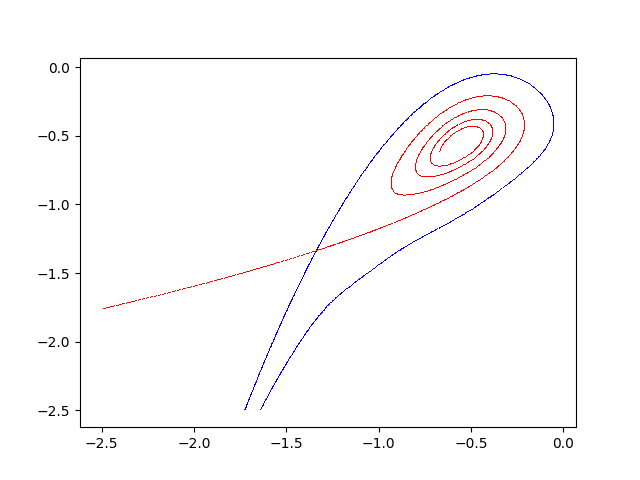
\includegraphics[width=6cm]{henon/b_less.png}}
		\subfigure[$b = -1$]{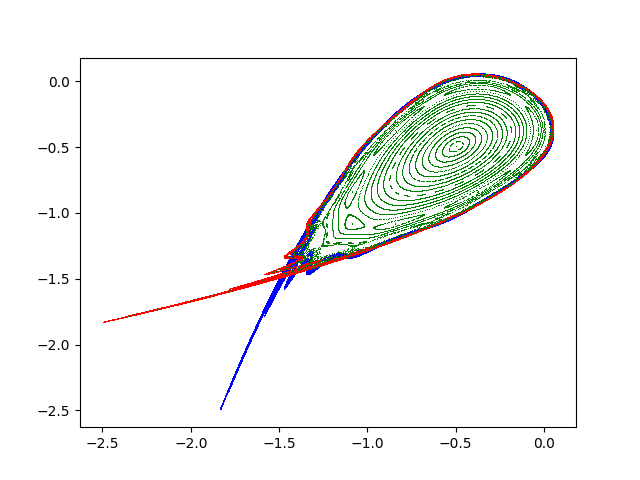
\includegraphics[width=6cm]{henon/b_one.png}}
		\subfigure[$b = -1,1$]{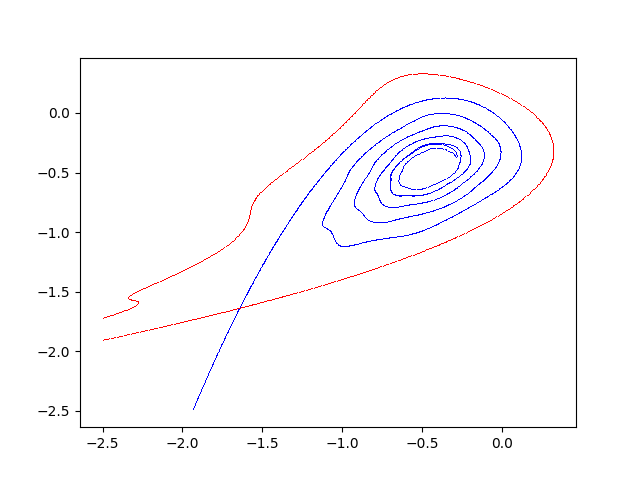
\includegraphics[width=6cm]{henon/b_more.png}}
	\end{figure}
	Percebe-se como as semelhan\c{c}as com as imagens do livro s\~ao satisfat\'orias.
	Pode-se perceber como para $|b| < 1$, a variedade inst\'avel est\'a em espiral sobre o
	ponto fixo. Como ela deve se afastar do ponto de sela, o ponto fixo dentro da espiral deve
	ser est\'avel. Para $|b| = 1$, observa-se exatamente quando o mapa \'e conservativo,
	com uma fam\'ilia de curvas invariantes aparecendo, mostradas em verdes, rodeada pelas
	variedades. Para $|b| > 1$, observa-se como a variedade est\'avel est\'a em espiral
	sobre o ponto fixo. Como ela deve se aproximar do ponto de sela, o ponto fixo
	dentro da espiral deve ser inst\'avel, provando como ele mudou de estabilidade.
	\section{Quest\~ao 3}
	Simplesmente gerando v\'arias \'orbitas a partir de um grid de pontos iniciais, tem-se:
	\begin{figure}[H]
		\centering
		\subfigure[$a = 0$]{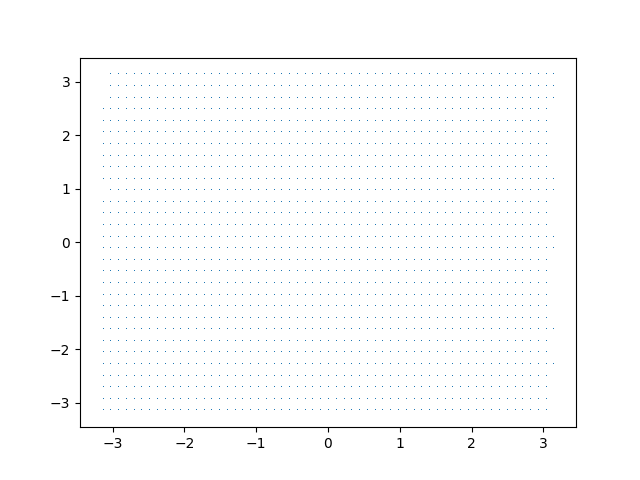
\includegraphics[width=6cm]{standard/standard0.png}}
		\subfigure[$a = 0,3$]{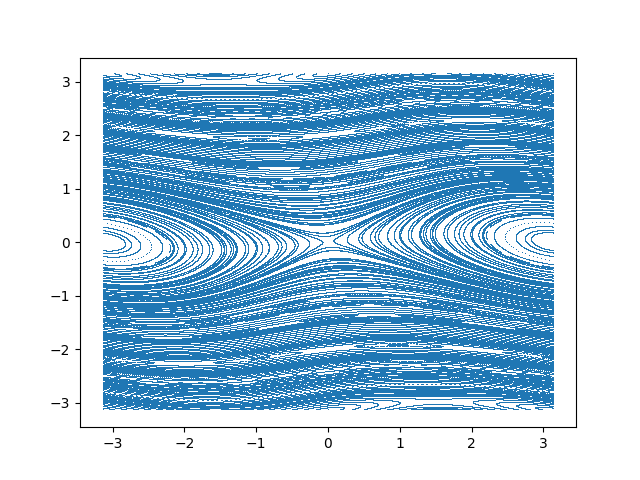
\includegraphics[width=6cm]{standard/standard03.png}}
		\subfigure[$a = 0,6$]{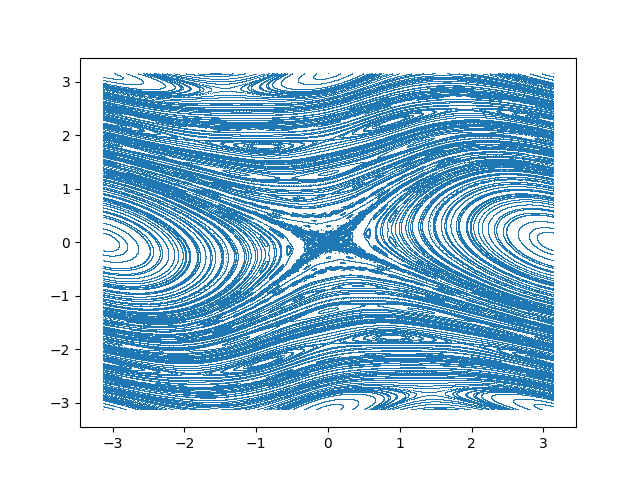
\includegraphics[width=6cm]{standard/standard06.png}}
		\subfigure[$a = 0,9$]{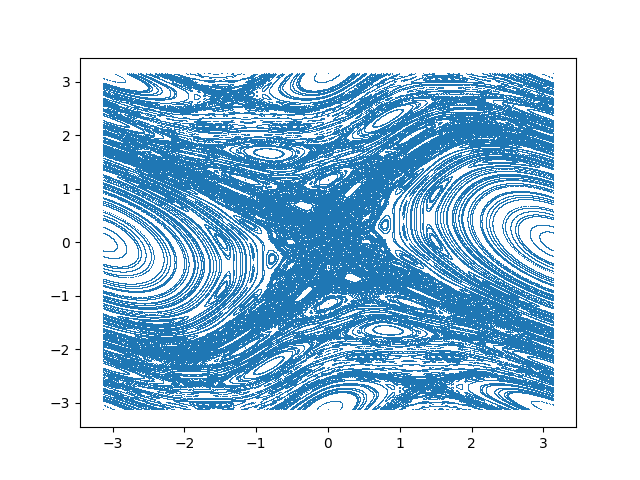
\includegraphics[width=6cm]{standard/standard09.png}}
		\subfigure[$a = 1,2$]{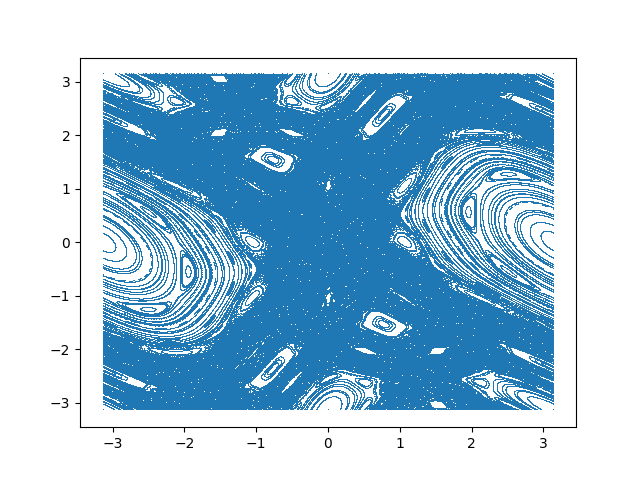
\includegraphics[width=6cm]{standard/standard12.png}}
		\subfigure[$a = 7$]{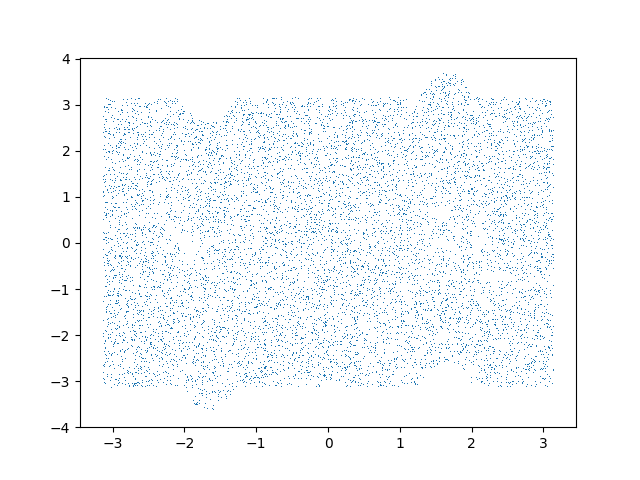
\includegraphics[width=6cm]{standard/standard7.png}}
	\end{figure}
	Onde se observam as curvas KAM, caracter\'isticas em mapas que preservam \'areas.
	A transforma\c{c}\~ao do espa\c{c}o em caos tamb\'em \'e evidente, e claramente
	s\~ao a mesma figura do livro, por\'em com resolu\c{c}\~ao maior. A \'ultima figura
	tamb\'em foi gerada com somente uma \'orbita, idem ao livro.
\end{document}
